\documentclass[1p]{elsarticle_modified}
%\bibliographystyle{elsarticle-num}

%\usepackage[colorlinks]{hyperref}
%\usepackage{abbrmath_seonhwa} %\Abb, \Ascr, \Acal ,\Abf, \Afrak
\usepackage{amsfonts}
\usepackage{amssymb}
\usepackage{amsmath}
\usepackage{amsthm}
\usepackage{scalefnt}
\usepackage{amsbsy}
\usepackage{kotex}
\usepackage{caption}
\usepackage{subfig}
\usepackage{color}
\usepackage{graphicx}
\usepackage{xcolor} %% white, black, red, green, blue, cyan, magenta, yellow
\usepackage{float}
\usepackage{setspace}
\usepackage{hyperref}

\usepackage{tikz}
\usetikzlibrary{arrows}

\usepackage{multirow}
\usepackage{array} % fixed length table
\usepackage{hhline}

%%%%%%%%%%%%%%%%%%%%%
\makeatletter
\renewcommand*\env@matrix[1][\arraystretch]{%
	\edef\arraystretch{#1}%
	\hskip -\arraycolsep
	\let\@ifnextchar\new@ifnextchar
	\array{*\c@MaxMatrixCols c}}
\makeatother %https://tex.stackexchange.com/questions/14071/how-can-i-increase-the-line-spacing-in-a-matrix
%%%%%%%%%%%%%%%

\usepackage[normalem]{ulem}

\newcommand{\msout}[1]{\ifmmode\text{\sout{\ensuremath{#1}}}\else\sout{#1}\fi}
%SOURCE: \msout is \stkout macro in https://tex.stackexchange.com/questions/20609/strikeout-in-math-mode

\newcommand{\cancel}[1]{
	\ifmmode
	{\color{red}\msout{#1}}
	\else
	{\color{red}\sout{#1}}
	\fi
}

\newcommand{\add}[1]{
	{\color{blue}\uwave{#1}}
}

\newcommand{\replace}[2]{
	\ifmmode
	{\color{red}\msout{#1}}{\color{blue}\uwave{#2}}
	\else
	{\color{red}\sout{#1}}{\color{blue}\uwave{#2}}
	\fi
}

\newcommand{\Sol}{\mathcal{S}} %segment
\newcommand{\D}{D} %diagram
\newcommand{\A}{\mathcal{A}} %arc


%%%%%%%%%%%%%%%%%%%%%%%%%%%%%5 test

\def\sl{\operatorname{\textup{SL}}(2,\Cbb)}
\def\psl{\operatorname{\textup{PSL}}(2,\Cbb)}
\def\quan{\mkern 1mu \triangleright \mkern 1mu}

\theoremstyle{definition}
\newtheorem{thm}{Theorem}[section]
\newtheorem{prop}[thm]{Proposition}
\newtheorem{lem}[thm]{Lemma}
\newtheorem{ques}[thm]{Question}
\newtheorem{cor}[thm]{Corollary}
\newtheorem{defn}[thm]{Definition}
\newtheorem{exam}[thm]{Example}
\newtheorem{rmk}[thm]{Remark}
\newtheorem{alg}[thm]{Algorithm}

\newcommand{\I}{\sqrt{-1}}
\begin{document}

%\begin{frontmatter}
%
%\title{Boundary parabolic representations of knots up to 8 crossings}
%
%%% Group authors per affiliation:
%\author{Yunhi Cho} 
%\address{Department of Mathematics, University of Seoul, Seoul, Korea}
%\ead{yhcho@uos.ac.kr}
%
%
%\author{Seonhwa Kim} %\fnref{s_kim}}
%\address{Center for Geometry and Physics, Institute for Basic Science, Pohang, 37673, Korea}
%\ead{ryeona17@ibs.re.kr}
%
%\author{Hyuk Kim}
%\address{Department of Mathematical Sciences, Seoul National University, Seoul 08826, Korea}
%\ead{hyukkim@snu.ac.kr}
%
%\author{Seokbeom Yoon}
%\address{Department of Mathematical Sciences, Seoul National University, Seoul, 08826,  Korea}
%\ead{sbyoon15@snu.ac.kr}
%
%\begin{abstract}
%We find all boundary parabolic representation of knots up to 8 crossings.
%
%\end{abstract}
%\begin{keyword}
%    \MSC[2010] 57M25 
%\end{keyword}
%
%\end{frontmatter}

%\linenumbers
%\tableofcontents
%
\newcommand\colored[1]{\textcolor{white}{\rule[-0.35ex]{0.8em}{1.4ex}}\kern-0.8em\color{red} #1}%
%\newcommand\colored[1]{\textcolor{white}{ #1}\kern-2.17ex	\textcolor{white}{ #1}\kern-1.81ex	\textcolor{white}{ #1}\kern-2.15ex\color{red}#1	}

{\Large $\underline{12n_{0304}~(K12n_{0304})}$}

\setlength{\tabcolsep}{10pt}
\renewcommand{\arraystretch}{1.6}
\vspace{1cm}\begin{tabular}{m{100pt}>{\centering\arraybackslash}m{274pt}}
\multirow{5}{120pt}{
	\centering
	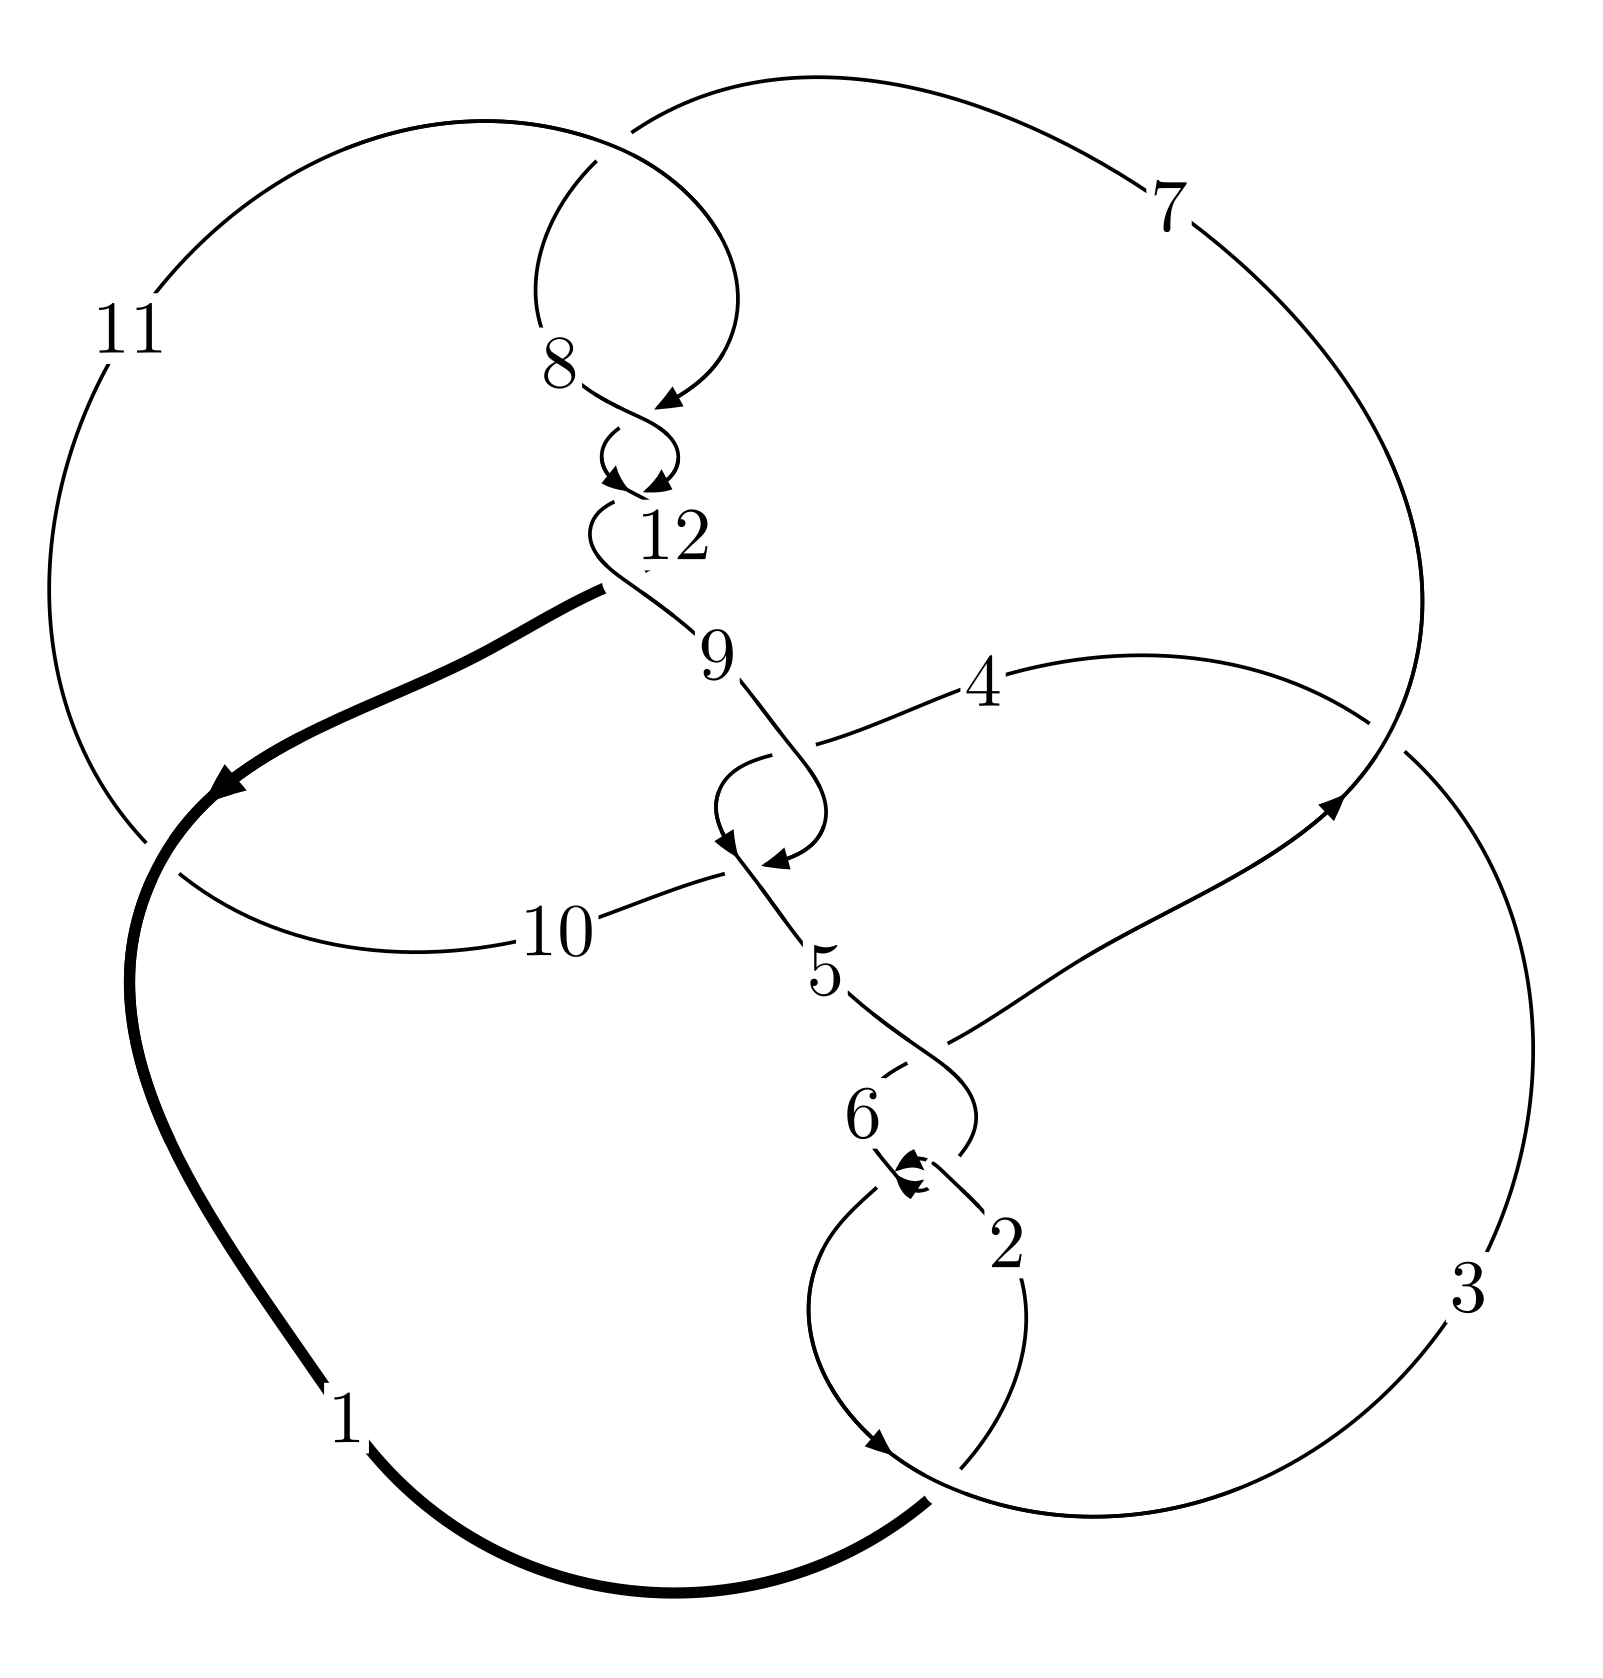
\includegraphics[width=112pt]{../../../GIT/diagram.site/Diagrams/png/2393_12n_0304.png}\\
\ \ \ A knot diagram\footnotemark}&
\allowdisplaybreaks
\textbf{Linearized knot diagam} \\
\cline{2-2}
 &
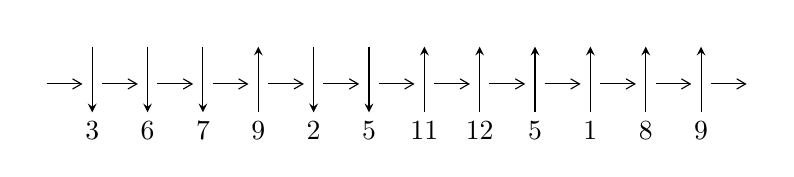
\begin{tikzpicture}[x=20pt, y=17pt]
	% nodes
	\node (C0) at (0, 0) {};
	\node (C1) at (1, 0) {};
	\node (C1U) at (1, +1) {};
	\node (C1D) at (1, -1) {3};

	\node (C2) at (2, 0) {};
	\node (C2U) at (2, +1) {};
	\node (C2D) at (2, -1) {6};

	\node (C3) at (3, 0) {};
	\node (C3U) at (3, +1) {};
	\node (C3D) at (3, -1) {7};

	\node (C4) at (4, 0) {};
	\node (C4U) at (4, +1) {};
	\node (C4D) at (4, -1) {9};

	\node (C5) at (5, 0) {};
	\node (C5U) at (5, +1) {};
	\node (C5D) at (5, -1) {2};

	\node (C6) at (6, 0) {};
	\node (C6U) at (6, +1) {};
	\node (C6D) at (6, -1) {5};

	\node (C7) at (7, 0) {};
	\node (C7U) at (7, +1) {};
	\node (C7D) at (7, -1) {11};

	\node (C8) at (8, 0) {};
	\node (C8U) at (8, +1) {};
	\node (C8D) at (8, -1) {12};

	\node (C9) at (9, 0) {};
	\node (C9U) at (9, +1) {};
	\node (C9D) at (9, -1) {5};

	\node (C10) at (10, 0) {};
	\node (C10U) at (10, +1) {};
	\node (C10D) at (10, -1) {1};

	\node (C11) at (11, 0) {};
	\node (C11U) at (11, +1) {};
	\node (C11D) at (11, -1) {8};

	\node (C12) at (12, 0) {};
	\node (C12U) at (12, +1) {};
	\node (C12D) at (12, -1) {9};
	\node (C13) at (13, 0) {};

	% arrows
	\draw[->,>={angle 60}]
	(C0) edge (C1) (C1) edge (C2) (C2) edge (C3) (C3) edge (C4) (C4) edge (C5) (C5) edge (C6) (C6) edge (C7) (C7) edge (C8) (C8) edge (C9) (C9) edge (C10) (C10) edge (C11) (C11) edge (C12) (C12) edge (C13) ;	\draw[->,>=stealth]
	(C1U) edge (C1D) (C2U) edge (C2D) (C3U) edge (C3D) (C4D) edge (C4U) (C5U) edge (C5D) (C6U) edge (C6D) (C7D) edge (C7U) (C8D) edge (C8U) (C9D) edge (C9U) (C10D) edge (C10U) (C11D) edge (C11U) (C12D) edge (C12U) ;
	\end{tikzpicture} \\
\hhline{~~} \\& 
\textbf{Solving Sequence} \\ \cline{2-2} 
 &
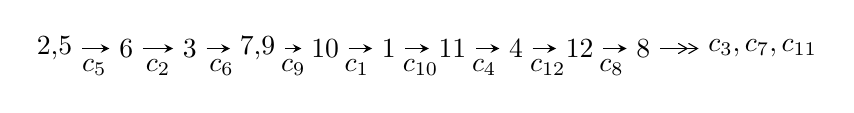
\begin{tikzpicture}[x=23pt, y=7pt]
	% node
	\node (A0) at (-1/8, 0) {2,5};
	\node (A1) at (1, 0) {6};
	\node (A2) at (2, 0) {3};
	\node (A3) at (49/16, 0) {7,9};
	\node (A4) at (33/8, 0) {10};
	\node (A5) at (41/8, 0) {1};
	\node (A6) at (49/8, 0) {11};
	\node (A7) at (57/8, 0) {4};
	\node (A8) at (65/8, 0) {12};
	\node (A9) at (73/8, 0) {8};
	\node (C1) at (1/2, -1) {$c_{5}$};
	\node (C2) at (3/2, -1) {$c_{2}$};
	\node (C3) at (5/2, -1) {$c_{6}$};
	\node (C4) at (29/8, -1) {$c_{9}$};
	\node (C5) at (37/8, -1) {$c_{1}$};
	\node (C6) at (45/8, -1) {$c_{10}$};
	\node (C7) at (53/8, -1) {$c_{4}$};
	\node (C8) at (61/8, -1) {$c_{12}$};
	\node (C9) at (69/8, -1) {$c_{8}$};
	\node (A10) at (11, 0) {$c_{3},c_{7},c_{11}$};

	% edge
	\draw[->,>=stealth]	
	(A0) edge (A1) (A1) edge (A2) (A2) edge (A3) (A3) edge (A4) (A4) edge (A5) (A5) edge (A6) (A6) edge (A7) (A7) edge (A8) (A8) edge (A9) ;
	\draw[->>,>={angle 60}]	
	(A9) edge (A10);
\end{tikzpicture} \\ 

\end{tabular} \\

\footnotetext{
The image of knot diagram is generated by the software ``\textbf{Draw programme}" developed by Andrew Bartholomew(\url{http://www.layer8.co.uk/maths/draw/index.htm\#Running-draw}), where we modified some parts for our purpose(\url{https://github.com/CATsTAILs/LinksPainter}).
}\phantom \\ \newline 
\centering \textbf{Ideals for irreducible components\footnotemark of $X_{\text{par}}$} 
 
\begin{align*}
I^u_{1}&=\langle 
-2 u^{40}-5 u^{39}+\cdots+b-2,\;2 u^{39}+5 u^{38}+\cdots+2 a-7,\;u^{41}+3 u^{40}+\cdots-4 u+1\rangle \\
I^u_{2}&=\langle 
b,\;a^2- a u- u^2+a+2 u-1,\;u^3- u^2+1\rangle \\
\\
\end{align*}
\raggedright * 2 irreducible components of $\dim_{\mathbb{C}}=0$, with total 47 representations.\\
\footnotetext{All coefficients of polynomials are rational numbers. But the coefficients are sometimes approximated in decimal forms when there is not enough margin.}
\newpage
\renewcommand{\arraystretch}{1}
\centering \section*{I. $I^u_{1}= \langle -2 u^{40}-5 u^{39}+\cdots+b-2,\;2 u^{39}+5 u^{38}+\cdots+2 a-7,\;u^{41}+3 u^{40}+\cdots-4 u+1 \rangle$}
\flushleft \textbf{(i) Arc colorings}\\
\begin{tabular}{m{7pt} m{180pt} m{7pt} m{180pt} }
\flushright $a_{2}=$&$\begin{pmatrix}0\\u\end{pmatrix}$ \\
\flushright $a_{5}=$&$\begin{pmatrix}1\\0\end{pmatrix}$ \\
\flushright $a_{6}=$&$\begin{pmatrix}1\\u^2\end{pmatrix}$ \\
\flushright $a_{3}=$&$\begin{pmatrix}- u\\- u^3+u\end{pmatrix}$ \\
\flushright $a_{7}=$&$\begin{pmatrix}- u^2+1\\u^2\end{pmatrix}$ \\
\flushright $a_{9}=$&$\begin{pmatrix}- u^{39}-\frac{5}{2} u^{38}+\cdots+4 u+\frac{7}{2}\\2 u^{40}+5 u^{39}+\cdots-12 u+2\end{pmatrix}$ \\
\flushright $a_{10}=$&$\begin{pmatrix}2 u^{40}+4 u^{39}+\cdots-8 u+\frac{11}{2}\\2 u^{40}+5 u^{39}+\cdots-12 u+2\end{pmatrix}$ \\
\flushright $a_{1}=$&$\begin{pmatrix}u^3\\u^5- u^3+u\end{pmatrix}$ \\
\flushright $a_{11}=$&$\begin{pmatrix}u^{40}+\frac{3}{2} u^{39}+\cdots-\frac{1}{2} u+4\\\frac{3}{2} u^{40}+\frac{9}{2} u^{39}+\cdots-\frac{21}{2} u+\frac{3}{2}\end{pmatrix}$ \\
\flushright $a_{4}=$&$\begin{pmatrix}u^7-2 u^5+2 u^3-2 u\\- u^7+u^5-2 u^3+u\end{pmatrix}$ \\
\flushright $a_{12}=$&$\begin{pmatrix}-\frac{1}{2} u^{38}- u^{37}+\cdots-6 u-\frac{1}{2}\\- u^{12}+2 u^{10}-4 u^8+4 u^6+2 u^5-3 u^4-2 u^3+2 u^2+2 u\end{pmatrix}$ \\
\flushright $a_{8}=$&$\begin{pmatrix}\frac{1}{2} u^{39}+u^{38}+\cdots+\frac{5}{2} u+2\\-\frac{1}{2} u^{40}-\frac{3}{2} u^{39}+\cdots+\frac{3}{2} u-\frac{1}{2}\end{pmatrix}$\\&\end{tabular}
\flushleft \textbf{(ii) Obstruction class $= -1$}\\~\\
\flushleft \textbf{(iii) Cusp Shapes $= -\frac{19}{2} u^{40}-20 u^{39}+\cdots+75 u-\frac{1}{2}$}\\~\\
\newpage\renewcommand{\arraystretch}{1}
\flushleft \textbf{(iv) u-Polynomials at the component}\newline \\
\begin{tabular}{m{50pt}|m{274pt}}
Crossings & \hspace{64pt}u-Polynomials at each crossing \\
\hline $$\begin{aligned}c_{1},c_{6}\end{aligned}$$&$\begin{aligned}
&u^{41}+15 u^{40}+\cdots+54 u+1
\end{aligned}$\\
\hline $$\begin{aligned}c_{2},c_{5}\end{aligned}$$&$\begin{aligned}
&u^{41}+3 u^{40}+\cdots-4 u+1
\end{aligned}$\\
\hline $$\begin{aligned}c_{3}\end{aligned}$$&$\begin{aligned}
&u^{41}-3 u^{40}+\cdots+2 u+1
\end{aligned}$\\
\hline $$\begin{aligned}c_{4},c_{9}\end{aligned}$$&$\begin{aligned}
&u^{41}- u^{40}+\cdots+32 u+64
\end{aligned}$\\
\hline $$\begin{aligned}c_{7},c_{8},c_{11}\\c_{12}\end{aligned}$$&$\begin{aligned}
&u^{41}-4 u^{40}+\cdots- u-1
\end{aligned}$\\
\hline $$\begin{aligned}c_{10}\end{aligned}$$&$\begin{aligned}
&u^{41}+6 u^{40}+\cdots-25 u-1
\end{aligned}$\\
\hline
\end{tabular}\\~\\
\newpage\renewcommand{\arraystretch}{1}
\flushleft \textbf{(v) Riley Polynomials at the component}\newline \\
\begin{tabular}{m{50pt}|m{274pt}}
Crossings & \hspace{64pt}Riley Polynomials at each crossing \\
\hline $$\begin{aligned}c_{1},c_{6}\end{aligned}$$&$\begin{aligned}
&y^{41}+25 y^{40}+\cdots+1814 y-1
\end{aligned}$\\
\hline $$\begin{aligned}c_{2},c_{5}\end{aligned}$$&$\begin{aligned}
&y^{41}-15 y^{40}+\cdots+54 y-1
\end{aligned}$\\
\hline $$\begin{aligned}c_{3}\end{aligned}$$&$\begin{aligned}
&y^{41}-35 y^{40}+\cdots+54 y-1
\end{aligned}$\\
\hline $$\begin{aligned}c_{4},c_{9}\end{aligned}$$&$\begin{aligned}
&y^{41}+35 y^{40}+\cdots-23552 y-4096
\end{aligned}$\\
\hline $$\begin{aligned}c_{7},c_{8},c_{11}\\c_{12}\end{aligned}$$&$\begin{aligned}
&y^{41}-46 y^{40}+\cdots- y-1
\end{aligned}$\\
\hline $$\begin{aligned}c_{10}\end{aligned}$$&$\begin{aligned}
&y^{41}+38 y^{40}+\cdots+419 y-1
\end{aligned}$\\
\hline
\end{tabular}\\~\\
\newpage\flushleft \textbf{(vi) Complex Volumes and Cusp Shapes}
$$\begin{array}{c|c|c}  
\text{Solutions to }I^u_{1}& \I (\text{vol} + \sqrt{-1}CS) & \text{Cusp shape}\\
 \hline 
\begin{aligned}
u &= -0.554966 + 0.821093 I \\
a &= \phantom{-}0.497003 - 1.229360 I \\
b &= -0.36616 + 1.39788 I\end{aligned}
 & -2.41826 - 3.80802 I & \phantom{-}3.60583 + 3.47707 I \\ \hline\begin{aligned}
u &= -0.554966 - 0.821093 I \\
a &= \phantom{-}0.497003 + 1.229360 I \\
b &= -0.36616 - 1.39788 I\end{aligned}
 & -2.41826 + 3.80802 I & \phantom{-}3.60583 - 3.47707 I \\ \hline\begin{aligned}
u &= -0.827605 + 0.515025 I \\
a &= -0.328705 + 0.303123 I \\
b &= -0.241607 + 0.924234 I\end{aligned}
 & \phantom{-}1.70931 + 2.07723 I & \phantom{-}4.47890 - 3.71404 I \\ \hline\begin{aligned}
u &= -0.827605 - 0.515025 I \\
a &= -0.328705 - 0.303123 I \\
b &= -0.241607 - 0.924234 I\end{aligned}
 & \phantom{-}1.70931 - 2.07723 I & \phantom{-}4.47890 + 3.71404 I \\ \hline\begin{aligned}
u &= \phantom{-}0.776023 + 0.578782 I \\
a &= \phantom{-}1.72542 + 0.58271 I \\
b &= -0.884835 + 0.226791 I\end{aligned}
 & \phantom{-}1.60480 - 0.80076 I & \phantom{-}5.09218 - 0.58482 I \\ \hline\begin{aligned}
u &= \phantom{-}0.776023 - 0.578782 I \\
a &= \phantom{-}1.72542 - 0.58271 I \\
b &= -0.884835 - 0.226791 I\end{aligned}
 & \phantom{-}1.60480 + 0.80076 I & \phantom{-}5.09218 + 0.58482 I \\ \hline\begin{aligned}
u &= -1.04869\phantom{ +0.000000I} \\
a &= \phantom{-}0.0572806\phantom{ +0.000000I} \\
b &= -1.17662\phantom{ +0.000000I}\end{aligned}
 & \phantom{-}3.30786\phantom{ +0.000000I} & \phantom{-}2.08440\phantom{ +0.000000I} \\ \hline\begin{aligned}
u &= -0.613160 + 0.856728 I \\
a &= -0.94977 + 1.28570 I \\
b &= \phantom{-}0.59049 - 1.37882 I\end{aligned}
 & \phantom{-}4.75528 - 6.89936 I & \phantom{-}6.92603 + 2.94505 I \\ \hline\begin{aligned}
u &= -0.613160 - 0.856728 I \\
a &= -0.94977 - 1.28570 I \\
b &= \phantom{-}0.59049 + 1.37882 I\end{aligned}
 & \phantom{-}4.75528 + 6.89936 I & \phantom{-}6.92603 - 2.94505 I \\ \hline\begin{aligned}
u &= -0.851706 + 0.644533 I \\
a &= \phantom{-}0.208645 - 1.142410 I \\
b &= \phantom{-}0.123688 - 0.806905 I\end{aligned}
 & \phantom{-}10.80640 + 2.51167 I & \phantom{-}3.89555 - 1.99801 I\\
 \hline 
 \end{array}$$\newpage$$\begin{array}{c|c|c}  
\text{Solutions to }I^u_{1}& \I (\text{vol} + \sqrt{-1}CS) & \text{Cusp shape}\\
 \hline 
\begin{aligned}
u &= -0.851706 - 0.644533 I \\
a &= \phantom{-}0.208645 + 1.142410 I \\
b &= \phantom{-}0.123688 + 0.806905 I\end{aligned}
 & \phantom{-}10.80640 - 2.51167 I & \phantom{-}3.89555 + 1.99801 I \\ \hline\begin{aligned}
u &= \phantom{-}0.607006 + 0.678640 I \\
a &= -2.19270 - 0.14272 I \\
b &= \phantom{-}1.058510 - 0.256762 I\end{aligned}
 & \phantom{-}8.39222 + 0.77239 I & \phantom{-}9.02070 + 0.54313 I \\ \hline\begin{aligned}
u &= \phantom{-}0.607006 - 0.678640 I \\
a &= -2.19270 + 0.14272 I \\
b &= \phantom{-}1.058510 + 0.256762 I\end{aligned}
 & \phantom{-}8.39222 - 0.77239 I & \phantom{-}9.02070 - 0.54313 I \\ \hline\begin{aligned}
u &= -0.468903 + 0.772766 I \\
a &= \phantom{-}0.050516 + 1.153690 I \\
b &= \phantom{-}0.094850 - 1.373440 I\end{aligned}
 & -2.97142 + 0.55275 I & \phantom{-}2.30390 - 2.65158 I \\ \hline\begin{aligned}
u &= -0.468903 - 0.772766 I \\
a &= \phantom{-}0.050516 - 1.153690 I \\
b &= \phantom{-}0.094850 + 1.373440 I\end{aligned}
 & -2.97142 - 0.55275 I & \phantom{-}2.30390 + 2.65158 I \\ \hline\begin{aligned}
u &= \phantom{-}0.917493 + 0.603542 I \\
a &= -1.30840 - 0.95232 I \\
b &= \phantom{-}0.987613 - 0.046245 I\end{aligned}
 & \phantom{-}1.14349 - 3.91148 I & \phantom{-}2.83783 + 7.19272 I \\ \hline\begin{aligned}
u &= \phantom{-}0.917493 - 0.603542 I \\
a &= -1.30840 + 0.95232 I \\
b &= \phantom{-}0.987613 + 0.046245 I\end{aligned}
 & \phantom{-}1.14349 + 3.91148 I & \phantom{-}2.83783 - 7.19272 I \\ \hline\begin{aligned}
u &= \phantom{-}1.145870 + 0.098490 I \\
a &= \phantom{-}0.557107 + 1.022870 I \\
b &= -0.43743 + 1.53434 I\end{aligned}
 & -1.90305 - 5.90674 I & \phantom{-}0.65317 + 3.76442 I \\ \hline\begin{aligned}
u &= \phantom{-}1.145870 - 0.098490 I \\
a &= \phantom{-}0.557107 - 1.022870 I \\
b &= -0.43743 - 1.53434 I\end{aligned}
 & -1.90305 + 5.90674 I & \phantom{-}0.65317 - 3.76442 I \\ \hline\begin{aligned}
u &= \phantom{-}1.150510 + 0.030891 I \\
a &= -0.178270 - 1.012240 I \\
b &= \phantom{-}0.13939 - 1.59211 I\end{aligned}
 & -8.52969 - 2.39687 I & -2.76728 + 3.02467 I\\
 \hline 
 \end{array}$$\newpage$$\begin{array}{c|c|c}  
\text{Solutions to }I^u_{1}& \I (\text{vol} + \sqrt{-1}CS) & \text{Cusp shape}\\
 \hline 
\begin{aligned}
u &= \phantom{-}1.150510 - 0.030891 I \\
a &= -0.178270 + 1.012240 I \\
b &= \phantom{-}0.13939 + 1.59211 I\end{aligned}
 & -8.52969 + 2.39687 I & -2.76728 - 3.02467 I \\ \hline\begin{aligned}
u &= \phantom{-}0.879522 + 0.766671 I \\
a &= \phantom{-}0.349468 - 0.635389 I \\
b &= -0.011712 + 0.469579 I\end{aligned}
 & \phantom{-}3.60760 - 2.89390 I & -5.91956 + 4.41976 I \\ \hline\begin{aligned}
u &= \phantom{-}0.879522 - 0.766671 I \\
a &= \phantom{-}0.349468 + 0.635389 I \\
b &= -0.011712 - 0.469579 I\end{aligned}
 & \phantom{-}3.60760 + 2.89390 I & -5.91956 - 4.41976 I \\ \hline\begin{aligned}
u &= -0.318016 + 0.760424 I \\
a &= -0.76042 - 1.22775 I \\
b &= \phantom{-}0.286457 + 1.371580 I\end{aligned}
 & \phantom{-}3.09276 + 3.48744 I & \phantom{-}6.36068 - 3.00060 I \\ \hline\begin{aligned}
u &= -0.318016 - 0.760424 I \\
a &= -0.76042 + 1.22775 I \\
b &= \phantom{-}0.286457 - 1.371580 I\end{aligned}
 & \phantom{-}3.09276 - 3.48744 I & \phantom{-}6.36068 + 3.00060 I \\ \hline\begin{aligned}
u &= -0.803311 + 0.150840 I \\
a &= \phantom{-}0.146401 - 0.020062 I \\
b &= \phantom{-}0.412782 - 0.447090 I\end{aligned}
 & -1.348790 + 0.350630 I & -5.34995 - 0.74571 I \\ \hline\begin{aligned}
u &= -0.803311 - 0.150840 I \\
a &= \phantom{-}0.146401 + 0.020062 I \\
b &= \phantom{-}0.412782 + 0.447090 I\end{aligned}
 & -1.348790 - 0.350630 I & -5.34995 + 0.74571 I \\ \hline\begin{aligned}
u &= -1.057040 + 0.554919 I \\
a &= -1.211900 - 0.182135 I \\
b &= -0.13020 + 1.48466 I\end{aligned}
 & \phantom{-}0.94110 + 1.27702 I & \phantom{-}2.95191 - 1.84094 I \\ \hline\begin{aligned}
u &= -1.057040 - 0.554919 I \\
a &= -1.211900 + 0.182135 I \\
b &= -0.13020 - 1.48466 I\end{aligned}
 & \phantom{-}0.94110 - 1.27702 I & \phantom{-}2.95191 + 1.84094 I \\ \hline\begin{aligned}
u &= \phantom{-}1.004470 + 0.646364 I \\
a &= \phantom{-}1.16107 + 1.33962 I \\
b &= -1.216110 - 0.239593 I\end{aligned}
 & \phantom{-}7.24069 - 5.93073 I & \phantom{-}6.53956 + 5.01754 I\\
 \hline 
 \end{array}$$\newpage$$\begin{array}{c|c|c}  
\text{Solutions to }I^u_{1}& \I (\text{vol} + \sqrt{-1}CS) & \text{Cusp shape}\\
 \hline 
\begin{aligned}
u &= \phantom{-}1.004470 - 0.646364 I \\
a &= \phantom{-}1.16107 - 1.33962 I \\
b &= -1.216110 + 0.239593 I\end{aligned}
 & \phantom{-}7.24069 + 5.93073 I & \phantom{-}6.53956 - 5.01754 I \\ \hline\begin{aligned}
u &= \phantom{-}0.891105 + 0.826186 I \\
a &= -0.68311 + 1.33083 I \\
b &= \phantom{-}0.038155 - 1.007650 I\end{aligned}
 & \phantom{-}10.04850 - 3.07313 I & \phantom{-}5.86480 + 2.85684 I \\ \hline\begin{aligned}
u &= \phantom{-}0.891105 - 0.826186 I \\
a &= -0.68311 - 1.33083 I \\
b &= \phantom{-}0.038155 + 1.007650 I\end{aligned}
 & \phantom{-}10.04850 + 3.07313 I & \phantom{-}5.86480 - 2.85684 I \\ \hline\begin{aligned}
u &= -1.066370 + 0.630817 I \\
a &= \phantom{-}1.70734 + 0.08552 I \\
b &= -0.22070 - 1.52920 I\end{aligned}
 & -4.70291 + 4.72137 I & \phantom{-0.000000 } 0. - 2.49884 I \\ \hline\begin{aligned}
u &= -1.066370 - 0.630817 I \\
a &= \phantom{-}1.70734 - 0.08552 I \\
b &= -0.22070 + 1.52920 I\end{aligned}
 & -4.70291 - 4.72137 I & \phantom{-0.000000 -}0. + 2.49884 I \\ \hline\begin{aligned}
u &= -1.067020 + 0.674301 I \\
a &= -2.03641 - 0.00933 I \\
b &= \phantom{-}0.45680 + 1.50432 I\end{aligned}
 & -3.95261 + 9.40997 I & \phantom{-}2.00000 - 7.76812 I \\ \hline\begin{aligned}
u &= -1.067020 - 0.674301 I \\
a &= -2.03641 + 0.00933 I \\
b &= \phantom{-}0.45680 - 1.50432 I\end{aligned}
 & -3.95261 - 9.40997 I & \phantom{-}2.00000 + 7.76812 I \\ \hline\begin{aligned}
u &= -1.061600 + 0.708976 I \\
a &= \phantom{-}2.31095 - 0.08552 I \\
b &= -0.65644 - 1.43319 I\end{aligned}
 & \phantom{-}3.38790 + 12.73300 I & \phantom{-}5.12799 - 7.34194 I \\ \hline\begin{aligned}
u &= -1.061600 - 0.708976 I \\
a &= \phantom{-}2.31095 + 0.08552 I \\
b &= -0.65644 + 1.43319 I\end{aligned}
 & \phantom{-}3.38790 - 12.73300 I & \phantom{-}5.12799 + 7.34194 I \\ \hline\begin{aligned}
u &= \phantom{-}0.530791\phantom{ +0.000000I} \\
a &= -3.58500\phantom{ +0.000000I} \\
b &= \phantom{-}0.511824\phantom{ +0.000000I}\end{aligned}
 & \phantom{-}8.14249\phantom{ +0.000000I} & \phantom{-}16.8230\phantom{ +0.000000I}\\
 \hline 
 \end{array}$$\newpage$$\begin{array}{c|c|c}  
\text{Solutions to }I^u_{1}& \I (\text{vol} + \sqrt{-1}CS) & \text{Cusp shape}\\
 \hline 
\begin{aligned}
u &= \phantom{-}0.153263\phantom{ +0.000000I} \\
a &= \phantom{-}3.39924\phantom{ +0.000000I} \\
b &= -0.382289\phantom{ +0.000000I}\end{aligned}
 & \phantom{-}0.765123\phantom{ +0.000000I} & \phantom{-}13.2670\phantom{ +0.000000I}\\
 \hline 
 \end{array}$$\newpage\newpage\renewcommand{\arraystretch}{1}
\centering \section*{II. $I^u_{2}= \langle b,\;a^2- a u- u^2+a+2 u-1,\;u^3- u^2+1 \rangle$}
\flushleft \textbf{(i) Arc colorings}\\
\begin{tabular}{m{7pt} m{180pt} m{7pt} m{180pt} }
\flushright $a_{2}=$&$\begin{pmatrix}0\\u\end{pmatrix}$ \\
\flushright $a_{5}=$&$\begin{pmatrix}1\\0\end{pmatrix}$ \\
\flushright $a_{6}=$&$\begin{pmatrix}1\\u^2\end{pmatrix}$ \\
\flushright $a_{3}=$&$\begin{pmatrix}- u\\- u^2+u+1\end{pmatrix}$ \\
\flushright $a_{7}=$&$\begin{pmatrix}- u^2+1\\u^2\end{pmatrix}$ \\
\flushright $a_{9}=$&$\begin{pmatrix}a\\0\end{pmatrix}$ \\
\flushright $a_{10}=$&$\begin{pmatrix}a\\0\end{pmatrix}$ \\
\flushright $a_{1}=$&$\begin{pmatrix}u^2-1\\- u^2\end{pmatrix}$ \\
\flushright $a_{11}=$&$\begin{pmatrix}- a u\\- u^2 a+a u+a\end{pmatrix}$ \\
\flushright $a_{4}=$&$\begin{pmatrix}1\\0\end{pmatrix}$ \\
\flushright $a_{12}=$&$\begin{pmatrix}u^2- a- u\\- u^2\end{pmatrix}$ \\
\flushright $a_{8}=$&$\begin{pmatrix}a u- u+1\\u^2 a- a u- a\end{pmatrix}$\\&\end{tabular}
\flushleft \textbf{(ii) Obstruction class $= 1$}\\~\\
\flushleft \textbf{(iii) Cusp Shapes $= u^2 a-3 u^2+a+8 u+7$}\\~\\
\newpage\renewcommand{\arraystretch}{1}
\flushleft \textbf{(iv) u-Polynomials at the component}\newline \\
\begin{tabular}{m{50pt}|m{274pt}}
Crossings & \hspace{64pt}u-Polynomials at each crossing \\
\hline $$\begin{aligned}c_{1},c_{3}\end{aligned}$$&$\begin{aligned}
&(u^3- u^2+2 u-1)^2
\end{aligned}$\\
\hline $$\begin{aligned}c_{2}\end{aligned}$$&$\begin{aligned}
&(u^3+u^2-1)^2
\end{aligned}$\\
\hline $$\begin{aligned}c_{4},c_{9}\end{aligned}$$&$\begin{aligned}
&u^6
\end{aligned}$\\
\hline $$\begin{aligned}c_{5}\end{aligned}$$&$\begin{aligned}
&(u^3- u^2+1)^2
\end{aligned}$\\
\hline $$\begin{aligned}c_{6}\end{aligned}$$&$\begin{aligned}
&(u^3+u^2+2 u+1)^2
\end{aligned}$\\
\hline $$\begin{aligned}c_{7},c_{8},c_{10}\end{aligned}$$&$\begin{aligned}
&(u^2- u-1)^3
\end{aligned}$\\
\hline $$\begin{aligned}c_{11},c_{12}\end{aligned}$$&$\begin{aligned}
&(u^2+u-1)^3
\end{aligned}$\\
\hline
\end{tabular}\\~\\
\newpage\renewcommand{\arraystretch}{1}
\flushleft \textbf{(v) Riley Polynomials at the component}\newline \\
\begin{tabular}{m{50pt}|m{274pt}}
Crossings & \hspace{64pt}Riley Polynomials at each crossing \\
\hline $$\begin{aligned}c_{1},c_{3},c_{6}\end{aligned}$$&$\begin{aligned}
&(y^3+3 y^2+2 y-1)^2
\end{aligned}$\\
\hline $$\begin{aligned}c_{2},c_{5}\end{aligned}$$&$\begin{aligned}
&(y^3- y^2+2 y-1)^2
\end{aligned}$\\
\hline $$\begin{aligned}c_{4},c_{9}\end{aligned}$$&$\begin{aligned}
&y^6
\end{aligned}$\\
\hline $$\begin{aligned}c_{7},c_{8},c_{10}\\c_{11},c_{12}\end{aligned}$$&$\begin{aligned}
&(y^2-3 y+1)^3
\end{aligned}$\\
\hline
\end{tabular}\\~\\
\newpage\flushleft \textbf{(vi) Complex Volumes and Cusp Shapes}
$$\begin{array}{c|c|c}  
\text{Solutions to }I^u_{2}& \I (\text{vol} + \sqrt{-1}CS) & \text{Cusp shape}\\
 \hline 
\begin{aligned}
u &= \phantom{-}0.877439 + 0.744862 I \\
a &= -0.198308 + 1.205210 I \\
b &= \phantom{-0.000000 } 0\end{aligned}
 & \phantom{-}11.90680 - 2.82812 I & \phantom{-}11.55793 + 3.24268 I \\ \hline\begin{aligned}
u &= \phantom{-}0.877439 + 0.744862 I \\
a &= \phantom{-}0.075747 - 0.460350 I \\
b &= \phantom{-0.000000 } 0\end{aligned}
 & \phantom{-}4.01109 - 2.82812 I & \phantom{-}14.0681 + 1.5771 I \\ \hline\begin{aligned}
u &= \phantom{-}0.877439 - 0.744862 I \\
a &= -0.198308 - 1.205210 I \\
b &= \phantom{-0.000000 } 0\end{aligned}
 & \phantom{-}11.90680 + 2.82812 I & \phantom{-}11.55793 - 3.24268 I \\ \hline\begin{aligned}
u &= \phantom{-}0.877439 - 0.744862 I \\
a &= \phantom{-}0.075747 + 0.460350 I \\
b &= \phantom{-0.000000 } 0\end{aligned}
 & \phantom{-}4.01109 + 2.82812 I & \phantom{-}14.0681 - 1.5771 I \\ \hline\begin{aligned}
u &= -0.754878\phantom{ +0.000000I} \\
a &= \phantom{-}1.08457\phantom{ +0.000000I} \\
b &= \phantom{-0.000000 } 0\end{aligned}
 & -0.126494\phantom{ +0.000000I} & \phantom{-}0.954070\phantom{ +0.000000I} \\ \hline\begin{aligned}
u &= -0.754878\phantom{ +0.000000I} \\
a &= -2.83945\phantom{ +0.000000I} \\
b &= \phantom{-0.000000 } 0\end{aligned}
 & \phantom{-}7.76919\phantom{ +0.000000I} & -5.20600\phantom{ +0.000000I}\\
 \hline 
 \end{array}$$\newpage
\newpage\renewcommand{\arraystretch}{1}
\centering \section*{ III. u-Polynomials}
\begin{tabular}{m{50pt}|m{274pt}}
Crossings & \hspace{64pt}u-Polynomials at each crossing \\
\hline $$\begin{aligned}c_{1}\end{aligned}$$&$\begin{aligned}
&((u^3- u^2+2 u-1)^2)(u^{41}+15 u^{40}+\cdots+54 u+1)
\end{aligned}$\\
\hline $$\begin{aligned}c_{2}\end{aligned}$$&$\begin{aligned}
&((u^3+u^2-1)^2)(u^{41}+3 u^{40}+\cdots-4 u+1)
\end{aligned}$\\
\hline $$\begin{aligned}c_{3}\end{aligned}$$&$\begin{aligned}
&((u^3- u^2+2 u-1)^2)(u^{41}-3 u^{40}+\cdots+2 u+1)
\end{aligned}$\\
\hline $$\begin{aligned}c_{4},c_{9}\end{aligned}$$&$\begin{aligned}
&u^6(u^{41}- u^{40}+\cdots+32 u+64)
\end{aligned}$\\
\hline $$\begin{aligned}c_{5}\end{aligned}$$&$\begin{aligned}
&((u^3- u^2+1)^2)(u^{41}+3 u^{40}+\cdots-4 u+1)
\end{aligned}$\\
\hline $$\begin{aligned}c_{6}\end{aligned}$$&$\begin{aligned}
&((u^3+u^2+2 u+1)^2)(u^{41}+15 u^{40}+\cdots+54 u+1)
\end{aligned}$\\
\hline $$\begin{aligned}c_{7},c_{8}\end{aligned}$$&$\begin{aligned}
&((u^2- u-1)^3)(u^{41}-4 u^{40}+\cdots- u-1)
\end{aligned}$\\
\hline $$\begin{aligned}c_{10}\end{aligned}$$&$\begin{aligned}
&((u^2- u-1)^3)(u^{41}+6 u^{40}+\cdots-25 u-1)
\end{aligned}$\\
\hline $$\begin{aligned}c_{11},c_{12}\end{aligned}$$&$\begin{aligned}
&((u^2+u-1)^3)(u^{41}-4 u^{40}+\cdots- u-1)
\end{aligned}$\\
\hline
\end{tabular}\newpage\renewcommand{\arraystretch}{1}
\centering \section*{ IV. Riley Polynomials}
\begin{tabular}{m{50pt}|m{274pt}}
Crossings & \hspace{64pt}Riley Polynomials at each crossing \\
\hline $$\begin{aligned}c_{1},c_{6}\end{aligned}$$&$\begin{aligned}
&((y^3+3 y^2+2 y-1)^2)(y^{41}+25 y^{40}+\cdots+1814 y-1)
\end{aligned}$\\
\hline $$\begin{aligned}c_{2},c_{5}\end{aligned}$$&$\begin{aligned}
&((y^3- y^2+2 y-1)^2)(y^{41}-15 y^{40}+\cdots+54 y-1)
\end{aligned}$\\
\hline $$\begin{aligned}c_{3}\end{aligned}$$&$\begin{aligned}
&((y^3+3 y^2+2 y-1)^2)(y^{41}-35 y^{40}+\cdots+54 y-1)
\end{aligned}$\\
\hline $$\begin{aligned}c_{4},c_{9}\end{aligned}$$&$\begin{aligned}
&y^6(y^{41}+35 y^{40}+\cdots-23552 y-4096)
\end{aligned}$\\
\hline $$\begin{aligned}c_{7},c_{8},c_{11}\\c_{12}\end{aligned}$$&$\begin{aligned}
&((y^2-3 y+1)^3)(y^{41}-46 y^{40}+\cdots- y-1)
\end{aligned}$\\
\hline $$\begin{aligned}c_{10}\end{aligned}$$&$\begin{aligned}
&((y^2-3 y+1)^3)(y^{41}+38 y^{40}+\cdots+419 y-1)
\end{aligned}$\\
\hline
\end{tabular}
\vskip 2pc
\end{document}